\documentclass[tikz,border=5pt]{standalone}

\usepackage{amsmath}
\usetikzlibrary{
    arrows.meta,
    calc,
    decorations.markings,
    angles,
    quotes
}

\begin{document}

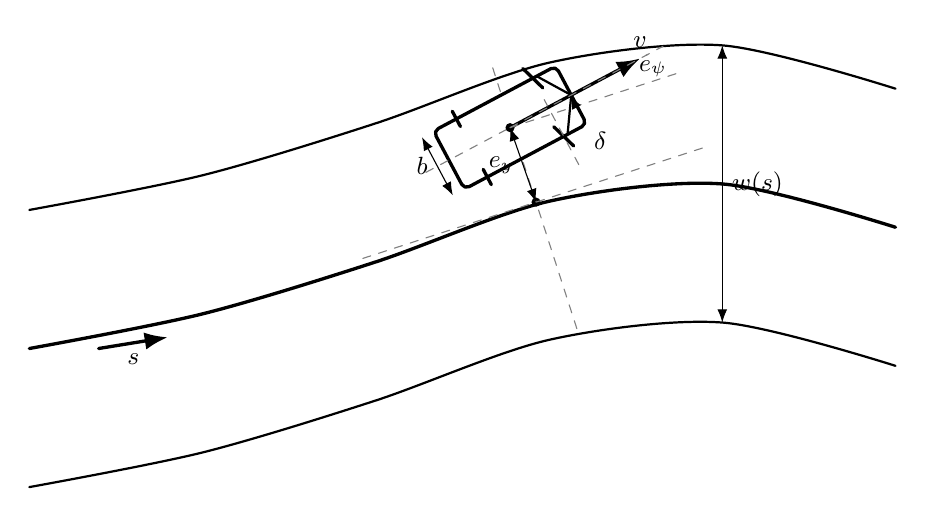
\begin{tikzpicture}[
    scale=1.1,
    >=Latex,
    line cap=round,
    line join=round,
    vector/.style={->, very thick},
    dimension/.style={<->, thin},
    dashed reference/.style={dashed, gray},
    every node/.style={font=\small}
]

% -------------------------------------------------
% Track geometry
% -------------------------------------------------

% Track centerline
\draw[very thick]
    plot[smooth] coordinates {
        (-5,-0.8)
        (-3,-0.4)
        (-1,0.2)
        (1,0.9)
        (3,1.1)
        (5,0.6)
    };

% Upper track boundary
\draw[thick]
    plot[smooth] coordinates {
        (-5,0.8)
        (-3,1.2)
        (-1,1.8)
        (1,2.5)
        (3,2.7)
        (5,2.2)
    };

% Lower track boundary
\draw[thick]
    plot[smooth] coordinates {
        (-5,-2.4)
        (-3,-2.0)
        (-1,-1.4)
        (1,-0.7)
        (3,-0.5)
        (5,-1.0)
    };

% Direction along the track
\draw[vector]
    (-4.2,-0.8) -- (-3.4,-0.67)
    node[midway, below] {$s$};

% -------------------------------------------------
% Reference point on centerline
% -------------------------------------------------

\coordinate (C) at (0.85,0.89);
\fill (C) circle (1.5pt);

% Tangent direction at C
\draw[dashed reference]
    ($(C)+(-2,-0.65)$) -- ($(C)+(2,0.65)$);

% Normal direction
\draw[dashed reference]
    ($(C)+(-0.5,1.55)$) -- ($(C)+(0.5,-1.55)$);

% -------------------------------------------------
% Vehicle
% -------------------------------------------------

\coordinate (V) at (0.55,1.75);

% Vehicle body, rotated relative to tangent
\begin{scope}[shift={(V)}, rotate=28]

    % Car body
    \draw[fill=white, very thick, rounded corners=2pt]
        (-0.8,-0.38) rectangle (0.8,0.38);

    % Front indication
    \draw[thick]
        (0.55,-0.38) -- (0.8,0)
        -- (0.55,0.38);

    % Rear wheels
    \draw[very thick]
        (-0.5,-0.48) -- (-0.5,-0.28);
    \draw[very thick]
        (-0.5,0.28) -- (-0.5,0.48);

    % Front wheels with steering angle
    \begin{scope}[shift={(0.5,-0.38)}, rotate=18]
        \draw[very thick] (0,-0.16) -- (0,0.16);
    \end{scope}

    \begin{scope}[shift={(0.5,0.38)}, rotate=18]
        \draw[very thick] (0,-0.16) -- (0,0.16);
    \end{scope}

    % Vehicle longitudinal axis
    \draw[dashed reference]
        (-1.1,0) -- (1.8,0);

    % Velocity vector
    \draw[vector]
        (0,0) -- (1.7,0)
        node[above] {$v$};

    % % Longitudinal acceleration
    % \draw[vector]
    %     (-0.1,-0.18) -- (1.2,-0.18)
    %     node[midway, below] {$a(t)$};

    % Car width
    \draw[dimension]
        (-0.95,-0.38) -- (-0.95,0.38)
        node[midway, left] {$b$};

    % Steering angle reference
    \draw[dashed reference]
        (0.5,-0.75) -- (0.5,0.1);


    \node at (0.85,-0.62) {$\delta$};

\end{scope}

% Vehicle reference point
\fill (V) circle (1.5pt);

% -------------------------------------------------
% Lateral error e_y
% -------------------------------------------------

\draw[dimension]
    ($(C)+(0,0)$)
    --
    ($(V)+(0,0)$)
    node[midway, left] {$e_y$};

% -------------------------------------------------
% Heading error e_psi
% -------------------------------------------------

% Approximate tangent reference direction from vehicle point
\draw[dashed reference]
    (V) -- ++(2,0.65);

% Vehicle heading reference
\draw[dashed reference]
    (V) -- ++({2*cos(28)},{2*sin(28)});

\draw[->]
    ($(V)+(0.75,0.24)$)
    arc[start angle=18,end angle=28,radius=0.8];

\node at ($(V)+(1.65,0.68)$) {$e_\psi$};

% -------------------------------------------------
% Track width
% -------------------------------------------------

\coordinate (WU) at (3,2.7);
\coordinate (WL) at (3,-0.5);

\draw[dimension]
    (WL) -- (WU)
    node[midway, right] {$w(s)$};


\end{tikzpicture}

\end{document}